\documentclass[11pt, english]{article}
\usepackage[a4paper, margin=2.5cm]{geometry}
\usepackage{graphicx} % Required for inserting images
\usepackage[useregional]{datetime2}
\usepackage{tabularx}

\usepackage{mathtools}
\DeclarePairedDelimiter{\ceil}{\lceil}{\rceil}

\begin{document}

\pagenumbering{gobble}% Remove page numbers (and reset to 1)
\thispagestyle{empty}
\begin{titlepage}
\begin{center}
  \centering
  
  \Huge \textbf{COMP3411 - Assignment 2} \\
  \vspace{5cm}
     
  \huge \textbf{Ryan McClue} \\
  (z5346008)
  \vspace{5cm}
    
  \today
\end{center}
\end{titlepage}

\section{Search Strategies for the 15-Puzzle}
\begin{table}[ht]
\centering
\begin{tabularx}{\linewidth}{X|X|X|X|X}
Start State & BFS & IDS & Greedy & A* \\\hline
start1 & 12, 10978 & 12, 25121 & 12, 59182 & 12, 30 \\
start2 & 17, 344890 & 17, 349380 & 17, 19  & 17, 35  \\
start3 & 18, 641252& 18, 1209934 & 22, 59196 & 18, 133 \\
\end{tabularx}
\end{table}
BFS is optimal when there are no weights, as is the case here.
Therefore, the length found will always be the smallest possible.
It's an uninformed search, which causes it to expand more nodes than necessary.
This can be seen comparing its number of expanded nodes with that of A*.
It has exponential space complexity.\\\\
IDS is optimal and uninformed like BFS. 
However, as it's a repeated DFS search, it will always expand more nodes than BFS.
This can be seen in comparing the expanded node count between IDS and BFS.
It has more efficient linear space complexity compared to BFS.\\\\
Greedy is suboptimal, meaning the length found may not always be the smallest possible.
This can be seen in start state 3.
It's an informed search, with a heuristic estimating the cost to the goal. 
So, it makes decisions in isolation, i.e. no thinking about past decisions.
As a result, it can potentially expand more nodes than an uninformed search as seen in start state 1.
Or, it could possibly expand less nodes as seen in start state 2.\\\\
A* is an informed search.
It uses a function that combines the cost of reaching the next node and a heuristic estimating cost to goal.
If this heuristic is admissable, i.e. doesn't overestimate cost, it's optimal.
In most cases, A* will expand the fewest nodes, as its guided by the most information.

\section{Heuristic Path Search for 15-Puzzle}
For $w=0$:
$$
f(n) = (2 - 0)g(n) + 0h(n) 
     = 2g(n)
$$
Scaling $g(n)$ by a constant factor has no effect on ordering of paths.
Therefore optimal.\\\\
For $w=1$:
$$
f(n) = (2 - 1)g(n) + 1h(n) 
     = g(n) + h(n)
$$
As $h(n)$ is admissable, know that this is optimal.
Therefore, optimal for $0 \leq w \leq 1$\\\\

\begin{table}[ht]
\centering
\begin{tabularx}{\linewidth}{X|X|X|X}
  & start4 & start5 & start6 \\\hline
IDA* Search & 45, 545120 & 50, 4178819 & 56, 169367641 \\
HPS, w=1.1   & 47, 523052 & 54, 857155  & 58, 13770561  \\
HPS, w=1.2   & 47, 29761  & 56, 64522   & 60, 265672    \\
HPS, w=1.3   & 55, 968    & 62, 5781    & 68, 9066      \\
HPS, w=1.4   & 65, 9876   & 70, 561430  & 80, 37869     \\
\end{tabularx}
\end{table}

For optimality, $h(n)$ must not overestimate, i.e. be admissable.
$w=1$ equates to IDA* search, which uses admissable heuristic.
Therefore, it is optimal and returns the smallest path length.
As values of $w$ increase, the greater extent $h(n)$ overestimates.
Therefore, as $w$ increases, optimality is reduced.
This can be seen for successive values of $w$ returning larger path lengths.

Larger values of $w$ make the function more greedy.
By making a function more greedy, we are most likely reducing the size of the decision space.
This equates to expanding less nodes.
For this particular problem, a certain level of greediness will reduce number of expanded nodes.
This is seen for searches up to $w=1.3$.
For $w=1.4$, number of expanded nodes begins to increase.
In general, greedy is more memory friendly, but less optimal.


\section{Graph Paper Grand Prix}
$M(1, 0) = [+,-] = 2$\\
$M(2, 0) = [+,o,-] = 3$\\
$M(3, 0) = [+,o,o,-] = 4$\\
$M(4, 0) = [+,+,-,-] = 4$\\
$M(5, 0) = [+,+,-,o,-] = 5$\\
$M(6, 0) = [+,+,o,-,-] = 5$\\
$M(7, 0) = [+,+,o,-,o,-] = 6$\\
$M(8, 0) = [+,+,o,o,-,-] = 6$\\
$M(9, 0) = [+,+,+,-,-,-] = 6$\\
$M(10, 0) = [+,+,+,-,-,o,-] = 7$\\
$M(11, 0) = [+,+,+,-,o,-,-] = 7$\\
$M(12, 0) = [+,+,+,o,-,-,-] = 7$\\
$M(13, 0) = [+,+,+,o,-,-,o,-] = 8$\\
$M(14, 0) = [+,+,+,o,-,o,-,-] = 8$\\
$M(15, 0) = [+,+,+,o,o,-,-,-] = 8$\\
$M(16, 0) = [+,+,+,+,-,-,-,-] = 8$\\
$M(17, 0) = [+,+,+,+,-,-,-,o,-] = 9$\\
$M(18, 0) = [+,+,+,+,-,-,o,-,-] = 9$\\
$M(19, 0) = [+,+,+,+,-,o,-,-,-] = 9$\\
$M(20, 0) = [+,+,+,+,o,-,-,-,-] = 9$\\
$M(21, 0) = [+,+,+,+,o,-,-,o,-] = 9$\\


Let $s$ be number of $+$ in a move sequence minus 1.
When $n$ is perfect square of $s$, i.e $n = (s + 1)^2$, $M = 2s + 2$.
Between successive $n$ terms that are perfect squares, the value of $M$ increases by 2.
So, between $s^2 \leq n \leq (s + 1)^2$ there will be 2 ranges to account for each single $M$ increment.
The range length is: $s^2 - (s + 1)^2 = 2s + 1$.
The first range is: $s^2 < n \leq s^2 + s$. 
This equates to $s^2 + k, 1 \leq k \leq s$
For this range, $M = 2s + 1$.
The second range is: $s^2 + s < n \leq (s+1)^2$. This equates to $s^2 + s + k, 1 \leq k \leq s$.
For this range, $M = 2s + 2$.
So, using the given identity, we have \ceil[\Big]{$2\sqrt{n}$}.\\

The distance travelled to reach velocity $k$ is given by arithmetic series:
$\frac{1}{2}k(k + 1)$
So, if we add this to $n$, i.e. $n' = n + \frac{1}{2}k(k + 1)$ we can use original formula $M(n', 0)$
However, this includes the number of steps to reach velocity $k$, when we are actually already starting at $k$.
So, subtract $k$ many moves.
So, $M(n, k) = M(n', 0) - k = \ceil[\Big]{$2\sqrt{n + \frac{1}{2}k(k + 1)$}} - k$
\\

If we consider the distance travelled to reach velocity $k$ as $\frac{1}{2}k(k + 1)$ and $n < \frac{1}{2}k(k - 1)$, the agent will go further than the goal.
So, will have to turn around and have negative velocity.
Therefore, first calculate distance to reach velocity $k$ and then reach negative velocity. 
This becomes:\\ 
$M(\frac{1}{2}k(k + 1) + \frac{1}{2}k(k - 1), 0)$\\
= \ceil[\Big]{$2\sqrt{\frac{1}{2}k(k + 1) + \frac{1}{2}k(k - 1)$}}\\
= \ceil[\Big]{$2\sqrt{\frac{k^2 + k + k^2 - k}{2}}$}\\
= \ceil[\Big]{$2\sqrt{k^2}$}\\
= \ceil[\Big]{2k}\\
= $2k$\\

Next have to travel back to $n$:\\
$M(\frac{1}{2}k(k - 1) - n, 0)$\\
= \ceil[\Big]{$2\sqrt{\frac{1}{2}k(k - 1) - n}$}\\

Finally, have to subtract $k$ as starting at $k$.
The final formula is:\\
$2k + \ceil[\Big]{$2\sqrt{\frac{1}{2}k(k - 1) - n}$} - k$\\
= $\ceil[\Big]{$2\sqrt{\frac{1}{2}k(k - 1) - n}$} + k$\\
\\\\
$h(r,c,u,v,r_G,c_G) = max(M(abs(r_G - r), u), M(abs(c_G - c), v))$\\
This heuristic is admissable as it only returns the distance in either the vertical or horizontal dimension.
As in 2D, one dimension will always be an underestimate.

\section{Game Trees and Pruning}
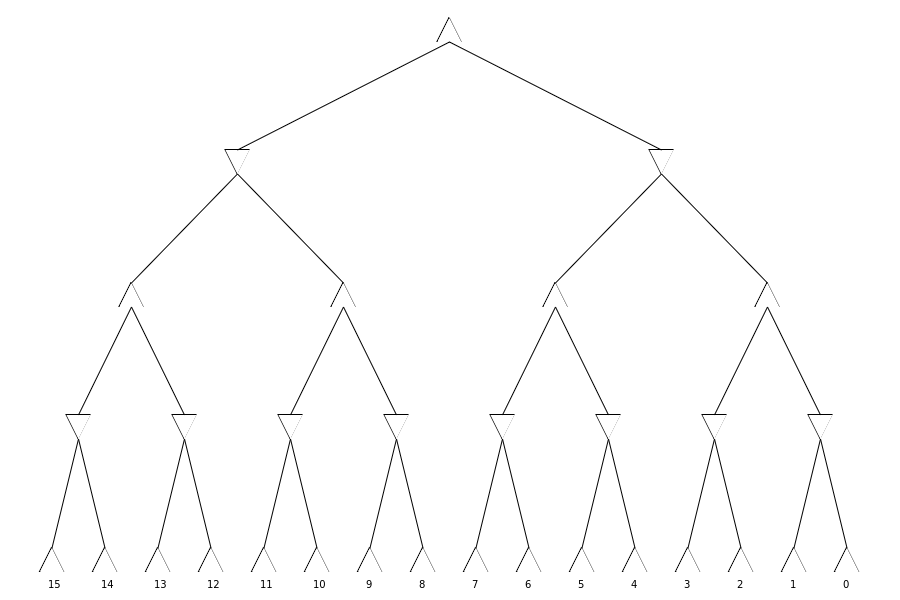
\includegraphics[width=1\textwidth]{minimax-tree.png}
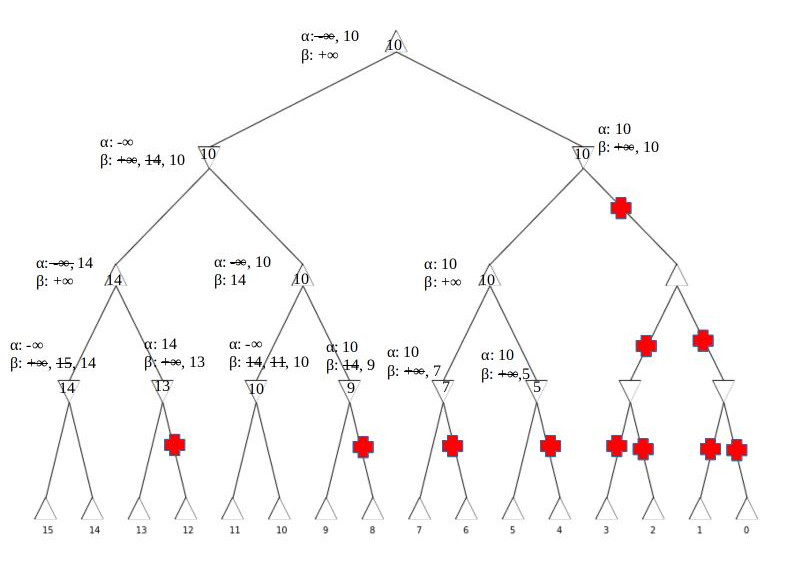
\includegraphics[width=1\textwidth]{pruned-tree-process.jpg}
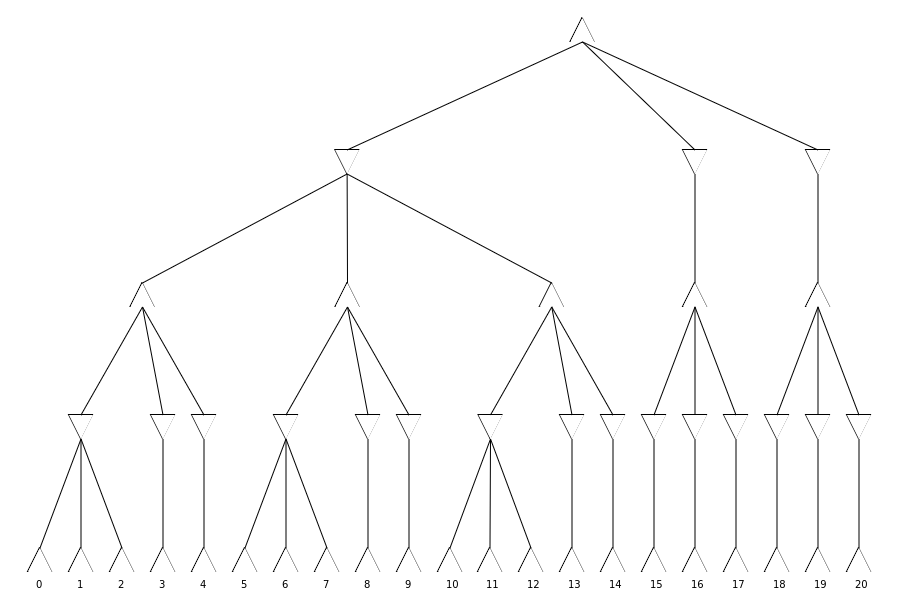
\includegraphics[width=1\textwidth]{pruned-tree-final.png}

4d.
Time complexity is
In the following analyses: 
b is the maximum branching factor in the search tree 
d is the depth of the least cost solution 
m is the maximum depth of the state space (may be infinity) 


\end{document}

